\documentclass[12pt,a4paper,UTF8]{ctexart}
\usepackage{graphicx}
\usepackage{amsmath}
\usepackage{amssymb}
\usepackage{cite}
\usepackage[ntheorem]{empheq}
\usepackage{enumitem}
\usepackage{fullpage}
\usepackage{tocbibind}
\usepackage[bookmarksopen=true,colorlinks,linkcolor=black]{hyperref}
\usepackage{cellspace}
\usepackage{listings}
\usepackage{color}
\usepackage{epstopdf}
\usepackage{subfigure}
\usepackage{algorithm}
\usepackage{algorithmicx}
\usepackage{algpseudocode}

\renewcommand{\algorithmicrequire}{\textbf{Input:}}  % Use Input in the format of Algorithm
\renewcommand{\algorithmicensure}{\textbf{Output:}} % Use Output in the format of Algorithm

\usepackage{longtable}

\usepackage{float}
\definecolor{gray}{rgb}{0.5,0.5,0.5}
\definecolor{dkgreen}{rgb}{.068,.578,.068}
\definecolor{dkpurple}{rgb}{.320,.064,.680}

% set Matlab styles
\lstset{
   language=Matlab,
   keywords={break,case,catch,continue,else,elseif,end,for,function,
      global,if,otherwise,persistent,return,switch,try,while},
   basicstyle=\ttfamily,
   keywordstyle=\color{blue}\bfseries,
   commentstyle=\color{dkgreen},
   stringstyle=\color{dkpurple},
   backgroundcolor=\color{white},
   tabsize=4,
   showspaces=false,
   showstringspaces=false
}

\begin{document}
\CJKfamily{zhkai}	


\begin{center}
\textbf{作业一}\\
\textbf{姓名\quad 徐家恒~~~~~~~~~~~~~ 学号 PB18000334~~~~~~~~~~~~~~ 日期 2021.	5.5}\\
\end{center}

\begin{center}
\fbox{
\begin{minipage}{40em}
\vspace{5cm}
\hspace{20cm}
\end{minipage}}
\end{center}
\vspace{1cm}

\begin{enumerate}
	\item[第一题]
	本题考虑使用有限差分方法(finite difference method)解决两点边值问题(boundary value problem)
	\begin{eqnarray*}
		-u^{\prime\prime}(x)=f(x)\quad(0<x<1)\text{使得}u(0)=T_0 \quad and\quad u(1)=T_1
	\end{eqnarray*}
	时产生的离散化线性系统
	\begin{eqnarray*}
		Ax=b
	\end{eqnarray*}	
	的求解问题。适当选取离散化的步长后我们会得到一个$10\times10$的系统:
	\begin{eqnarray*}
		A=\left[\begin{array}{llllll}
			2   & -1 &        &        &    &    \\
	        -1  & 2  & -1     &        &    &    \\
           		& -1 & 2      & \ddots &    &    \\
            	&    & \ddots & \ddots & -1 &    \\
            	&    &        & -1     & 2  & -1 \\
            	&    &        &        & -1 & 2
		\end{array}\right],\quad
		b=\left[\begin{array}{rrrrrrrrrr}
        	2 & -2 & 2 & -1 & 0 & 0 & 1 & -2 & 2 & -2
		\end{array}\right]^T
	\end{eqnarray*}
	此处,A中空白部分的元素皆为0。我们容易验证上述线性系统的精确解为
	\begin{eqnarray}\label{eq:1}
		x_{exact}=\left[\begin{array}{cccccccccc}
       		1 & 0 & 1 & 0 & 0 & 0 & 0 & -1 & 0 & -1
		\end{array}\right]^T
	\end{eqnarray}
	(a) (20分)分别使用Jacobi和Gauss-Siedel方法求解上述问题。利用精确解\eqref{eq:1}将误差大小和迭代次数的关系用semilogy图表示出来 (横轴为迭代次数 $n$, 纵轴为迭代解与精确解的差距)。


	semilogy图见下图\ref{jpg:1}\\

	(b) (10分)选取若干不同的松他因子 $\omega$ 使用SOR方法解上述问题,并将收敛结果画在上一问的图中。请在图上相应的收敛线旁标示出这些 $\omega$ 的值。以迭代次数做为判断标准,指出对应于$10 ^{-15}$ 的误差目标哪个大概的 $\omega$ 值收敛速度最快。\\
	

	收敛结果如下图\ref{jpg:1},由图可知$\omega \approx 1.6$时收敛速度最快

	\begin{figure}[H]
		\centering
     	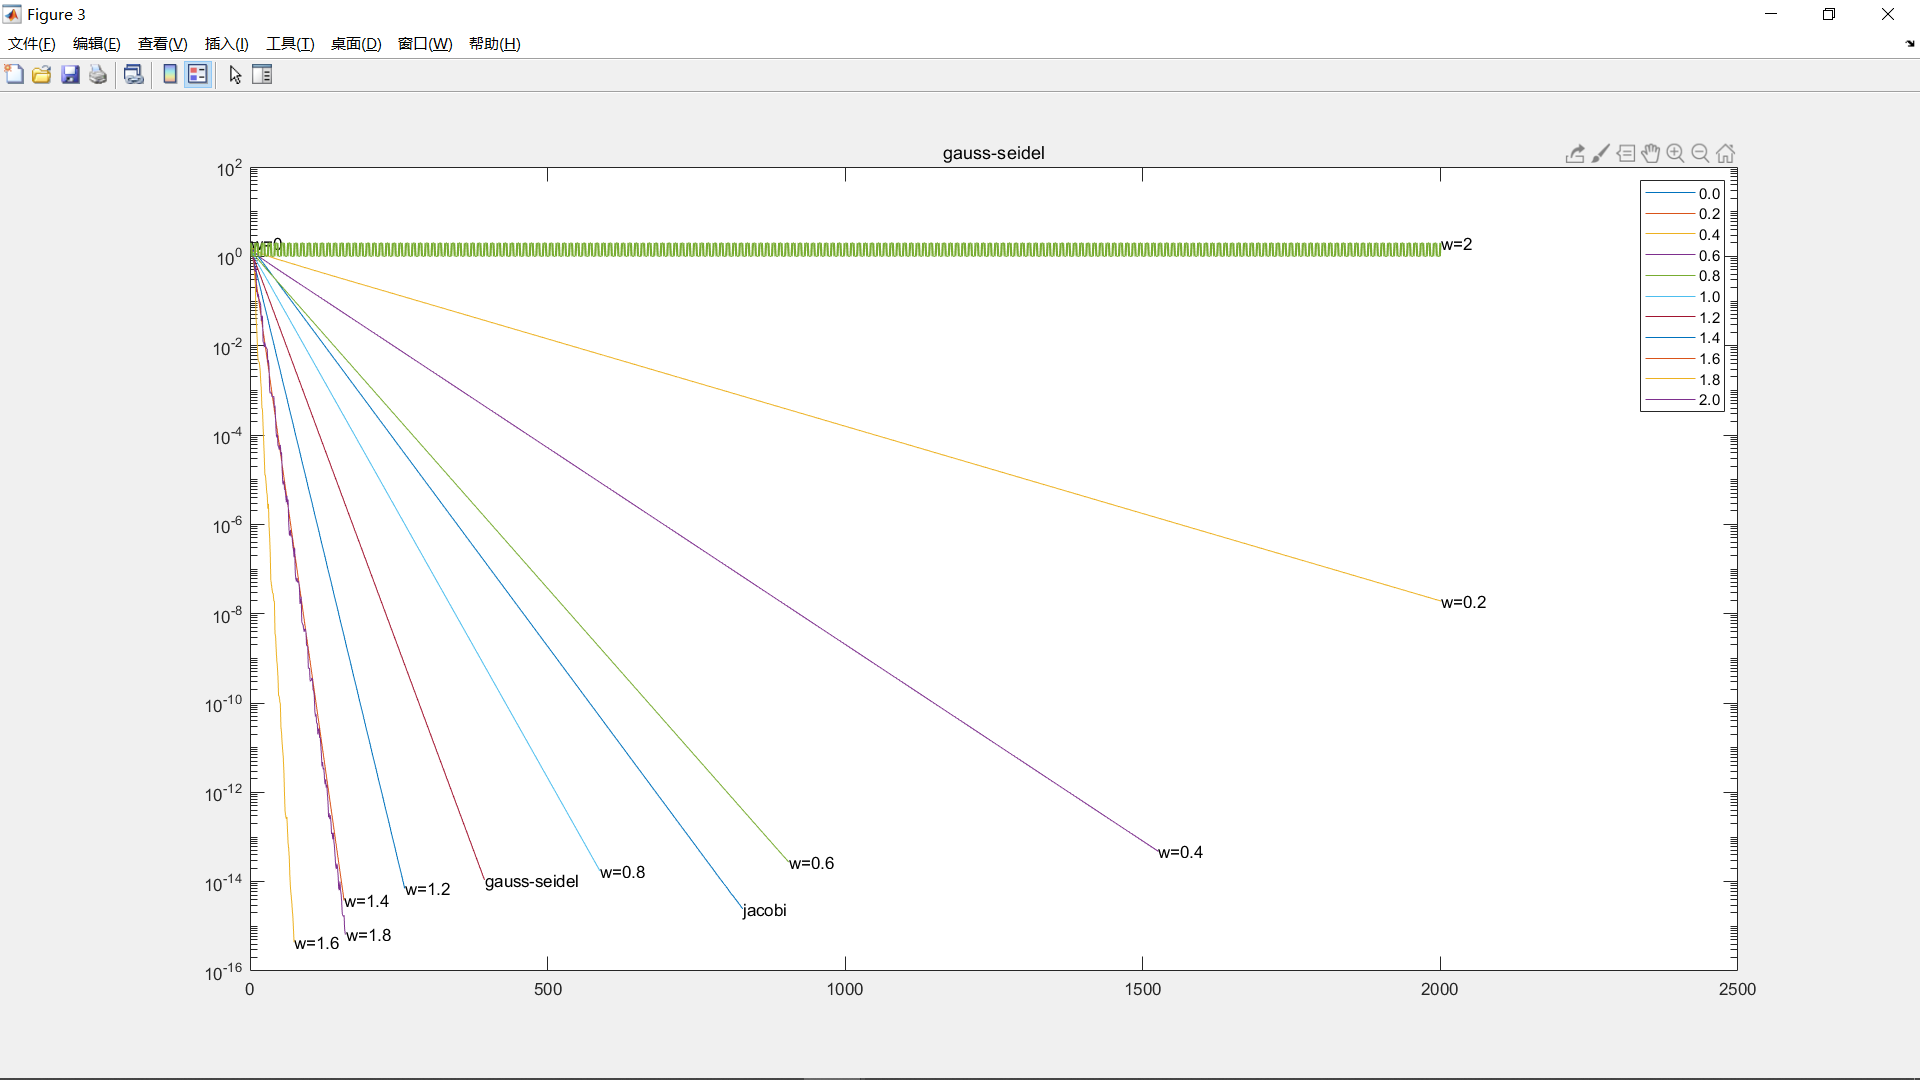
\includegraphics[width=0.8\textwidth]{1.png}
    	\caption{误差大小与迭代次数的semilogy图}\label{jpg:1}
	\end{figure}
	
	\begin{lstlisting}[frame=single,numbers=left] 
clc
%init
A = [
2 -1 0 0 0 0 0 0 0 0;
-1 2 -1 0 0 0 0 0 0 0;
0 -1 2 -1 0 0 0 0 0 0;
0 0 -1 2 -1 0 0 0 0 0;
0 0 0 -1 2 -1 0 0 0 0;
0 0 0 0 -1 2 -1 0 0 0;
0 0 0 0 0 -1 2 -1 0 0;
0 0 0 0 0 0 -1 2 -1 0;
0 0 0 0 0 0 0 -1 2 -1;
0 0 0 0 0 0 0 0 -1 2;
];
b = [2 -2 2 -1 0 0 1 -2 2 -2].';
exact = [1 0 1 0 0 0 0 -1 0 -1].';

[~,n] = size(A);
normInf = max(abs(exact));
vecNorm = zeros(1,1);

L = tril(A,-1);
D = diag(diag(A));
U = triu(A,1);
I = eye(n);
%precision
epsilon = 1e-15;

%jacobi
k = 0;
while norm(x1 - x2,inf)>epsilon
    x1 = x2;
    x2 = R * x1 + g;
    k = k + 1;
    vecNorm(k) = max(abs(x2 - exact))/normInf;
end

figure
semilogy(vecNorm)
text(k,vecNorm(k),'jacobi');
hold on
%w-gauss-seidel
for w = 0.0:0.2:2.0
    x1 = zeros(n,1);
    x2 = ones(n,1);
    vecNorm = zeros(1,1);
    
    k = 0;
    S = (I + w * (D\L))\((1 - w) * I - w * (D\U));
    f = w * ((I + w * (D\L))\(D\b));
    while norm(x1 - x2,inf)>epsilon
        x1 = x2;
        x2 = S * x1 + f;
        k = k + 1;
        vecNorm(k) = max(abs(x2 - exact))/normInf;
        if k>2000
            break;
        end
    end
    if w==1
        text(k,vecNorm(k),'gauss-seidel');
    else
        text(k,vecNorm(k),['w=',num2str(w)]);
    end
    semilogy(vecNorm)
    hold on
end
legend('0.0','0.2','0.4','0.6','0.8','1.0','1.2','1.4','1.6','1.8','2.0');

title('gauss-seidel');
	\end{lstlisting}
	(c) (15分)注意到题目中的矩阵A是一个稀疏矩阵(sparse matrix),即有大量元素为0的矩阵。更改你的程序,省略那些和零元素相关的运算,使得你的程序得到加速。使用MATLAB中的tic和toc命令统计上述三种方法得到较为精确的解的时候的计算用时,并和改进后的程序的(在使用相同迭代次数的情况下的)耗时列表做对比(左边一列为未加速的程序的计算时间,右边一列为加速后的时间)。注意你需要将每种方法反复运行$N$次(比如10次)然后忽略第一次的运行时间,求后面 $N-1$ 次运行时间的平均值或者总和。这是由于MATLAB需要在第一次运算时对程序进行编译并分 配存储空间。这类花费被统称为overhead, 中文有时会勉强地将其译为“额外开销"。\\
          \begin{table}[H]
              \centering
              \begin{tabular}{|c|c|c|}
                  \hline
             
                  Jacobi                    & 0.0012518889                 & 0.0011993333                    \\ \hline
                  Gauss-Siedel              & 0.0005258173                    & 0.0007343235                 \\ \hline
                  SOR $\omega$=1.6          & 0.0001674235              & 0.0002052688                   \\ \hline
              \end{tabular}
		\end{table}

		除jacobi外均为负优化,说明matlab本身对矩阵运算有优化处理

	jacobi优化:

\begin{lstlisting}[frame=single,numbers=left]
while norm(x1 - x2, inf)>epsilon
    x1 = x2;
    x2(1) = R(1, 2) * x1(2) + g(1);
    x2(10) = R(10, 9) * x1(9) + g(10);
    for i = 2:9
        x2(i) = R(i, i - 1) * x1(i - 1) + R(i, i + 1) * x1(i + 1) + g(i);
    end
    k = k + 1;
    vecNorm(k) = max(abs(x2 - exact))/normInf;
end
\end{lstlisting}

gauss seidel优化
\begin{lstlisting}[frame=single,numbers=left]
while norm(x1 - x2,inf)>epsilon
    x1 = x2;
    for i = 1:9
        x2(i) = f(i);
        for j = 2:i + 1
            x2(i) = x2(i) + S(i, j) * x1(j);
        end
    end
    x2(10) = f(10);
    for j = 2:10
        x2(10) = x2(10) + S(10, j) * x1(j);
    end
    k = k + 1;
    vecNorm(k) = max(abs(x2 - exact))/normInf;
end
\end{lstlisting}

sor w优化
\begin{lstlisting}[frame=single,numbers=left]    
while norm(x1 - x2,inf)>epsilon
    x1 = x2;
    for i = 1:9
        x2(i) = f(i);
        for j = 1:i + 1
            x2(i) = x2(i) + S(i, j) * x1(j);
        end
    end
    x2(10) = f(10);
    for j = 1:10
        x2(10) = x2(10) + S(10, j) * x1(j);
    end
    x2 = x2 + f;
    k = k + 1;
    vecNorm(k) = max(abs(x2 - exact))/normInf;
end
\end{lstlisting}


	\item[第二题]
	本题将利用求解方程
	\begin{eqnarray}\label{eq:2}
		x^3-3x^2+2=0
	\end{eqnarray}
	的根来深入我们关于Newton方法的收敛速度的讨论。容易验证\eqref{eq:2}的三个根分别位于$[-3,0]$、$[0,2]$、$[2,4]$三个区间内。我们依从左向右的顺序分别称这三个根为$x_l$、$x_m$、$x_r$。

	(a) (10分)适当选取迭代的初始点,写程序用Newton法求解这三个根,并将每
一步迭代的新的近似值打印出来。

	(b) (10分)设计一个估计收敛阶数的方法,在上一问求解的过程中同时求出大概的收敛阶数。

	本题采用的方法是
	\begin{eqnarray*}
		order\approx \frac{\log \left|\left(x_{n+1}-x_{n}\right) /\left(x_{n}-x_{n-1}\right)\right|}{\log \left|\left(x_{n}-x_{n-1}\right) /\left(x_{n-1}-x_{n-2}\right)\right|} 
	\end{eqnarray*}
\begin{table}[H]
\centering
\begin{tabular}{|l|l|l|}
\hline
k & x1                 & order             \\ \hline
1 & -0.777777777777778 &                   \\ \hline
2 & -0.733756613756614 & 1.000000000000000 \\ \hline
3 & -0.732053321730378 & 2.008704671554972 \\ \hline
4 & -0.732050807574351 & 2.004355840939773 \\ \hline
5 & -0.732050807568877 & 2.000099949796975 \\ \hline
6 & -0.732050807568877 & 2.000000074224094 \\ \hline
\end{tabular}
\caption{x1=-1}
\end{table}
\begin{table}[H]
\centering
\begin{tabular}{|l|l|l|}
\hline
k & x2                & order             \\ \hline
1 & 0.999326599326599 &                   \\ \hline
2 & 1.000000000203577 & 1.000000000000000 \\ \hline
3 & 1.000000000000000 & 2.997986296007438 \\ \hline
4 & 1.000000000000000 & 2.999999969792531 \\ \hline
\end{tabular}
\caption{x1=1.1}
\end{table}
\begin{table}[H]
\centering
\begin{tabular}{|l|l|l|}
\hline
k & x3                & order             \\ \hline
1 & 2.777777777777778 &                   \\ \hline
2 & 2.733756613756614 & 1.000000000000000 \\ \hline
3 & 2.732053321730378 & 2.008704671554972 \\ \hline
4 & 2.732050807574351 & 2.004355840939773 \\ \hline
5 & 2.732050807568877 & 2.000099949796975 \\ \hline
6 & 2.732050807568877 & 2.000000074224094 \\ \hline
\end{tabular}
\caption{x1=3}
\end{table}

	\begin{lstlisting}[frame=single,numbers=left]
clc;
syms x;
epsilon = 1e-15;
x1 = -1;
x2 = 1.1;
x3 = 3;
maxrept = 1000;
f(x) = x.^3 - 3 * x.^2 + 2;

fprintf('%10s  %20s  %20s\n','k','x1','order');
res = newton1(f, x1, epsilon, maxrept);
fprintf('\n ans  = %20.15f\n\n', res);
fprintf('%10s  %20s  %20s\n','k','x2','order');
res = newton1(f, x2, epsilon, maxrept);
fprintf('\n ans  = %20.15f\n\n', res);
fprintf('%10s  %20s  %20s\n','k','x3','order');
res = newton1(f, x3, epsilon, maxrept);
fprintf('\n ans  = %20.15f\n\n', res);

function x2 = newton1(f, x0, epsilon, maxrept)
    syms x;
    g(x) = diff(f, x);
    x1 = x0 - f(x0)/g(x0);
    x2 = x1 - f(x1)/g(x1);
    order0 = log(abs(x2 - x1)/abs(x1 - x0));
    fprintf('%10d  %20.15f\n',1 ,x1);
    for k = 2:maxrept
        x2 = x1 - f(x1)/g(x1);
        order1 = order0;
        order0 = log(abs(x2 - x1)/abs(x1 - x0));
        x0 = x1;
        x1 = x2;
        fprintf('%10d  %20.15f  %20.15f\n',k ,x2, order0/order1);
        if abs(x1 - x0) < epsilon
            break;
        end
    end
end
	\end{lstlisting}
	(c) (10分)Newton是一个二阶收敛的方法。上一问中你是否观测到了比二阶收
敛更快的现象?如果有,请尽可能详细地解释其原因。\\
	
	求$x_m$时,收敛阶$q\approx 3$\\

	由泰勒展开有\\

$0=f(x)=f(x_n)+(x-x_n)f^\prime(x_n)+\frac{(x-x_n)^2}{2}f^{\prime \prime}(x_n)$\\

此时有$\frac{x-x_n}{(x-x_n)^2}=-\frac{f^{\prime \prime}(x_n)}{2f^\prime(x_n)}$,收敛阶为2\\

在$x_m=1$附近,有$f^{\prime \prime}(x_m)=(6x-6)\rvert_{x=1}=0$\\

此时方程变为$0=f(x)=f(x_n)+(x-x_n)f^\prime(x_n)+\frac{(x-x_n)^2}{2}f^{\prime \prime}(x_n)+\frac{(x-x_n)^3}{6}f^{\prime \prime \prime}(x_n)$\\

此时有$\frac{x-x_n}{(x-x_n)^3}=-\frac{f^{\prime \prime \prime}(x_n)}{6f^\prime(x_n)}$,收敛阶为3\\

	\item[第三题]
	我们已经学习了使用幂法求解特征值问题。

	(a) (15分)设计一个能够求解问题存在一个(绝对值意义下的)最大特征值和
存在最大的两个特征值,大小相同但符号相反的情况的算法并仿照课堂上所
介绍的伪代码的格式写出一个清晰易懂的伪代码。\\

	$for \quad k = 1 \quad to\quad maxrept$
	
	\quad $Y^{k}=X^{k}/\lVert X^{k}\rVert_\infty$

	\quad $X^{k+1}=A*Y^{k}$

	\quad $if \quad \lVert X^{k}-X^{k+1}\rVert < \epsilon$

	\quad \quad $\lambda = \underset{1\le i\le n}{max} \lvert X^{k+1}_i \rvert$

	\quad \quad $\boldsymbol{vec} = Y^k$

	\quad $elseif \quad \lVert X^{k}+X^{k+1}\rVert < \epsilon$

	\quad \quad $\lambda = \underset{1\le i\le n}{max} \lvert X^{k+1}_i \rvert$

	\quad \quad $\boldsymbol{vec} = Y^k$

	\quad $endif$

	\quad $X^k=X^{k+1}$

	$end$


	(b) (10分)用程序实现上一问中你设计的算法,用于求解          
		\begin{equation}
        	A=\left[\begin{array}{rrrr}
      	      -148 & -105 & -83  & -67  \\
       	       488  & 343  & 269  & 216  \\
    	       -382 & -268 & -210 & -170 \\
     	         50   & 38   & 32   & 29
            \end{array}\right]
       	\end{equation}
	的模最大的特征值和特征向量(你提供的特征向量的 $\infty$ -范数应为1)。如果用你的程序求一 $A$ 的模最大的特征值和特征向量呢?你需要保证你的程序对负值的特征值也有效。

	\begin{lstlisting}[frame=single,numbers=left]
	clc;


A = [-148, -105, -83, -67
    488, 343, 269, 216
    -382, -268, -210, -170
    50, 38, 32, 29];
%A = -A;
[~,n] = size(A);
Xk = ones(n, 1);
maxrept = 1000;
epsilon = 1e-14;


lamda2 = 0;
lamda3 = 0;
for k = 2:maxrept
    Xk1 = A * Xk;
    lamda0 = max(abs(Xk1));
    Xk1 = Xk1/norm(Xk1,inf);
    Xk2 = A * Xk1;
    lamda1 = max(abs(Xk2));
    if abs(lamda0 - lamda1) < epsilon
        fprintf('\nlamda = %20.15f\n', sqrt(lamda0));
        Xk1
        break
    elseif abs(lamda0 + lamda1) < epsilon
        fprintf('\nlamda1 = %20.15f\n', -sqrt(lamda0));
        Xk1
        break
    elseif abs(lamda0 - lamda3) < epsilon && abs(lamda1 - lamda2) < epsilon
        Xk = Xk2;
        Xk2 = A * Xk2;
        lamda0 = sqrt(Xk2(1)/Xk1(1));
        lamda1 = -lamda0;
        fprintf('\nlamda1 = %20.15f\n', lamda0);
        Xk1 = Xk2 + lamda0 * Xk;
        Xk1 = Xk1/norm(Xk1,inf);
        Xk1
        fprintf('\nlamda2 = %20.15f\n', lamda1);
        Xk1 = Xk2 - lamda0 * Xk;
        Xk1 = Xk1/norm(Xk1,inf);
        Xk1
        break
    end
    Xk = Xk1;
    Xk1 = Xk2;
    lamda2 = lamda0;
    lamda3 = lamda1;
    fprintf('%7d  %20.15f\n', k, lamda1);
end
	\end{lstlisting}

	由上程序可得,在误差范围$\epsilon = 1e-14$内\\

	A的特征值
	$\lambda = 8.000000000000600$

	A的特征向量
	$	\boldsymbol{x}=\left(\begin{array}{c}
  -0.310344827586207\\
   1.000000000000000\\
  -0.793103448275861\\
   0.137931034482757\end{array}\right)$\\

	-A的特征值
	$\lambda = 8.000000000000600$

	-A的特征向量
	$	\boldsymbol{x}=\left(\begin{array}{c}
  -0.310344827586207\\
   1.000000000000000\\
  -0.793103448275861\\
   0.137931034482757\end{array}\right)$

	(c) (10分)用程序实现第一问中你设计的算法,用于求解
	$\left(\begin{array}{c}
                      -1.000000000000000 \\
                      0.285714285714289  \\
                      -0.178571428571430 \\
                      0.214285714285712
     \end{array}\right)$\\

	的模最大的特征值和特征向量(你提供的特征向量的$\infty$-范数应为1)。\\
	
		由上程序可得,在误差范围$\epsilon = 1e-14$内\\

	特征值1
	$\lambda_1 = 5.000000000000078$

	特征向量1
	$	\boldsymbol{x_1}=\left(\begin{array}{c}
    1.000000000000000\\
  -0.499999999999967\\
   0.125000000000011\\
  -0.0000000000000317\end{array}\right)$\\

	特征值2
	$\lambda_2 = -5.000000000000078$

	特征向量2
	$	\boldsymbol{x_1}=\left(\begin{array}{c}
   1.000000000000000\\
  -0.333333333333334\\
   0.166666666666667\\
  -0.166666666666666\end{array}\right)$\\

	(d) (10分)在Matlab中设定随机数种子为rng(2)使用rand命令生成一个100×
100的随机矩阵。用你的程序求解离$0.8 - 0.6i$最近的特征值和特征向量(你
提供的特征向量的∞-范数应为1)。\\

	程序如下,求得离$0.8-0.6i$最近的\\
	特征值$\lambda = 0.854519917670556 - 0.662123265348281i$

	迭代过程\\

\begin{longtable}{c|c}
\caption{迭代过程}\label{tab1}
 

\endfirsthead
 
\multicolumn{2}{c}{k}{norm}\
\endhead
 
\multicolumn{2}{c}{Continued on next page}
\endfoot
\endlastfoot
 
 
% 表格内容
k  & norm               \\ \hline
2  & 1.564456721915273  \\ \hline
3  & 12.284284873453794 \\ \hline
4  & 2.773657227732159  \\ \hline
5  & 8.431498212095160  \\ \hline
6  & 3.108946897196919  \\ \hline
7  & 7.946870702079942  \\ \hline
8  & 3.169896419852224  \\ \hline
9  & 7.871473317328734  \\ \hline
10 & 3.179902050131084  \\ \hline
11 & 7.859436240318765  \\ \hline
12 & 3.181511306997918  \\ \hline
13 & 7.857509858925735  \\ \hline
14 & 3.181769071462289  \\ \hline
15 & 7.857201580880184  \\ \hline
16 & 3.181810323780105  \\ \hline
17 & 7.857152253108357  \\ \hline
18 & 3.181816924516828  \\ \hline
19 & 7.857144360506751  \\ \hline
20 & 3.181817980648835  \\ \hline
21 & 7.857143097683308  \\ \hline
22 & 3.181818149630177  \\ \hline
23 & 7.857142895630996  \\ \hline
24 & 3.181818176667379  \\ \hline
25 & 7.857142863303157  \\ \hline
26 & 3.181818180993170  \\ \hline
27 & 7.857142858131390  \\ \hline
28 & 3.181818181685183  \\ \hline
29 & 7.857142857302956  \\ \hline
30 & 3.181818181795850  \\ \hline
31 & 7.857142857171601  \\ \hline
32 & 3.181818181813334  \\ \hline
33 & 7.857142857150085  \\ \hline
34 & 3.181818181816474  \\ \hline
35 & 7.857142857146568  \\ \hline
36 & 3.181818181817083  \\ \hline
37 & 7.857142857145701  \\ \hline
38 & 3.181818181817683  \\ \hline
39 & 7.857142857144874  \\ \hline
40 & 3.181818181816993  \\ \hline
41 & 7.857142857145393  \\ \hline
42 & 3.181818181817145  \\ \hline
43 & 7.857142857144916  \\ \hline
44 & 3.181818181816965  \\ \hline
45 & 7.857142857145300  \\ \hline
46 & 3.181818181816996  \\ \hline
47 & 7.857142857145311  \\ \hline
48 & 3.181818181817738  \\ \hline
49 & 7.857142857144931  \\ \hline
50 & 3.181818181817039  \\ \hline
51 & 7.857142857144669  \\ \hline
52 & 3.181818181816693  \\ \hline
53 & 7.857142857146027  \\ \hline
54 & 3.181818181816936  \\ \hline
55 & 7.857142857145095  \\ \hline
56 & 3.181818181816883  \\ \hline
57 & 7.857142857147086  \\ \hline
58 & 3.181818181816547  \\ \hline
59 & 7.857142857146782  \\ \hline
60 & 3.181818181816296  \\ \hline
61 & 7.857142857147373  \\ \hline
62 & 3.181818181816334  \\ \hline
63 & 7.857142857147121  \\ \hline
64 & 3.181818181816781  \\ \hline
65 & 7.857142857146171  \\ \hline
66 & 3.181818181817474  \\ \hline
67 & 7.857142857144632  \\ \hline
68 & 3.181818181816884  \\ \hline
69 & 7.857142857145929  \\ \hline
70 & 3.181818181816563  \\ \hline
71 & 7.857142857147668  \\ \hline
72 & 3.181818181816984  \\ \hline
73 & 7.857142857146254  \\ \hline
74 & 3.181818181816424  \\ \hline
75 & 7.857142857146878  \\ \hline
76 & 3.181818181816745  \\ \hline
77 & 7.857142857147156  \\ \hline
78 & 3.181818181816302  \\ \hline
79 & 7.857142857147337  \\ \hline
80 & 3.181818181816104  \\ \hline
81 & 7.857142857147995  \\ \hline
82 & 3.181818181815588  \\ \hline
83 & 7.857142857149115  \\ \hline
84 & 3.181818181816241  \\ \hline
85 & 7.857142857147361  \\ \hline
86 & 3.181818181816517  \\ \hline
87 & 7.857142857146804  \\ \hline
88 & 3.181818181816071  \\ \hline
89 & 7.857142857148382  \\ \hline
90 & 3.181818181816013  \\ \hline
91 & 7.857142857148790  \\ \hline
92 & 3.181818181815713  \\ \hline
93 & 7.857142857148988  \\ \hline
\end{longtable}
	\begin{lstlisting}[numbers=left,frame=single]
clc;
rng(2)
A = rand(100);
[~,n] = size(A);
Xk = ones(n, 1);
maxrept = 1000;
epsilon = 1e-15;

p = 0.8 - 0.6i;
[L,U] = lu(A - p * eye(100));
mu1 = 0;
for k = 2:maxrept
    Xk1 = U\(L\Xk);
    Xk1 = Xk1/norm(Xk1,2);
    mu0 = dot(Xk1, A * Xk1);
    if abs(mu0 - mu1) < epsilon
        mu0
        Xk1;
        break
    end
    mu1 = mu0;
    Xk = Xk1;
    fprintf('%7d  %20.15f\n', k, mu0);
end
	\end{lstlisting}
\end{enumerate}
\end{document}